\chapter{Metriche}\label{ch:chapter1}

Le protagoniste della nostra analisi sono, come anticipato nell'introduzione: 
\textbf{Improved Precision and Recall}, \textbf{Density and Coverage}, \textbf{Probabilistic Precision and Recall} e \textbf{Precision and Recall Cover}. 
Saranno poi introdotte tecniche più recenti come la \textbf{Precision Recall Curve} e altre metriche correlate.\
Tutte le metriche citate hanno una serie di caratteristiche in comune, il primo è forse più ovvio è che sono citate in coppia. 
Queste coppie cercano infatti di misurare due aspetti complementari delle reti generative: la \textbf{Fidelity} e la \textbf{Diversity}. 
Il secondo aspetto verrà discusso e approfondito invece nelle sezioni seguenti ed è relativo a come queste metriche sono misurate. Ciascuna di esse infatti 
si basa su un calcolo simile dipendente dalla distanza tra campioni generati e reali e la distanza \textbf{interset} vale a dire fra campioni vicini di uno stesso insieme.
E utile definire meglio dei concetti appena accennati: 
\begin{itemize}
    \item \textbf{Fidelity}: è la somiglianza tra i campioni generati e quelli reali.
    \item \textbf{Diversity}: è la varietà tra i campioni generati.
    \item \textbf{Precision}: misura la proporzione di campioni generati che ricadono nel supporto della distribuzione reale.
    \item \textbf{Recall}: misura la proporzione di campioni reali che ricadono nel supporto della distribuzione generata.
\end{itemize}
Sebbene \textit{fidelity} e \textit{diversity} siano concetti centraliper la valutazione della qualità dei modelli generativi, risultano difficili da quantificare direttamente a causa della loro natura astratta.
Si riduce quindi il problema del calcolo della \textit{fidelity} e \textit{diversity} a quello del calcolo della \textit{precision} e \textit{recall} (che offrono una formalizzazione più operativa di questi concetti, fornendo una base matematica per una valutazione quantitativa).
Entrambe si basano sul concetto di \textbf{supporto} della distribuzione. Dato un numero limitato di campioni, definire un supporto continuo è un problema non banale. 
Le diverse metriche si limitano a dare diverse stime di tale supporto. In questo contesto la stima del supporto è detto \textbf{manifold}.\

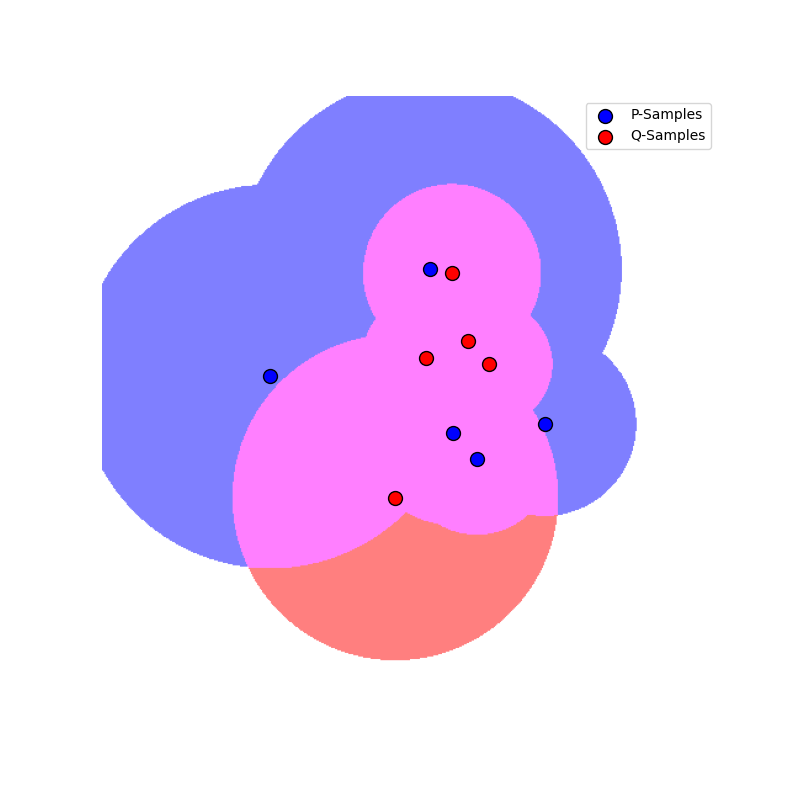
\includegraphics[width=\linewidth]{../manifold.png}

\section{Improved Precision and Recall}
\label{sec:improved-precision-and-recall}

Nonostante sia nominalmente dichiarato come "Improved" Precision Recall e quindi sottointendendo un miglioramento ad una versione meno 'potente' di Precision Recall, 
in realtà la metrica proposta da Sajjadi et al. \cite{sajjadi2018assessing} è antecendente a quella che verrà presentata in seguito (chiamata più semplicemente Precision Recall Cover)
ed è quindi la forma più semplice di Precision Recall che analizzeremo e dalla quale partiremo.

Sia $R$ il dataset reale e $G$ il dataset generato, identifichiamo con $\Phi_R$ e $\Phi_G$ le caratteristiche estratte da $R$ e $G$ rispettivamente.
Il manifold stimato da $R$ e $G$ è un insieme di ipersfere con un certo raggio e centrate nei vari putni di $\Phi_R$ e $\Phi_G$. Il raggio di queste ipersfere è 
determinato da un iperparametro $k$ che rappresenta il numero dei \textit{nearest neighbors} da considerare. Possiamo quindi definire una funzione binaria che 
determini se un certo punto appartiene al manifold o meno:
\begin{equation}
    f_{ipr}(x, \Phi) = 
    \begin{cases}
        1 & \text{if }~~ \exists ~ y \in \Phi \text{ such that } ||x - y||_2 \leq ||y - NN_k(y, \Phi)||_2 \\
        0 & \text{otherwise.}
    \end{cases}
\end{equation}

Dove $NN_k(y, \Phi)$ è il $k$-th nearest neighbor di $y$ in $\Phi$.

La Precision e la Recall possono essere quindi definite come:
\begin{equation}
    Precision(\Phi_R, \Phi_G) = \frac{1}{|\Phi_G|} \sum_{g \in \Phi_G} f_{ipr}(g, \Phi_R)
\end{equation}
\begin{equation}
    Recall(\Phi_R, \Phi_G) = \frac{1}{|\Phi_R|} \sum_{r \in \Phi_R} f_{ipr}(r, \Phi_G)
\end{equation}

Come ripeteremo in seguito la metrica risulta dipendente dall'iperparametro $k$ e in particolare pare che per $k=3$ si ottengano i risultati migliori.

\section{Density and Coverage}
\label{sec:density-and-coverage}

Come vedremo in seguito l'Improved Precision Recall soffre la presenza di outliers nei datasets, vale a dire che il manifold stimato da $R$ e $G$ può essere fortemente influenzato da pochi punti molto distanti dalla distribuzione principale.
La Density and Coverage è una metrica che cerca di mitigare questo problema. Invece che contare se le varie ipersfere in $\Phi_R$ contengono almeno un punto di $\Phi_G$ si conta quanti punti di $\Phi_G$ sono contenuti in ciascuna ipersfera di $\Phi_R$.
Questo conporta però che la density non è una metrica normalizzata e in certi casi assume valori maggiori di 1. 
\begin{equation}
    Density(\Phi_R, \Phi_G) = \frac{1}{k|\Phi_G|} \sum_{g \in \Phi_G} \sum_{r \in \Phi_R} \mathbbm{1}_{||r - g||_2 \leq ||g - NN_k(g, \Phi_G)||_2}
\end{equation}

Rispetto alle altre metriche in cui si poteva apprezzare la simmetria fra le formule per la stima di fidelity e diversity, in questo caso la Coverage è una metrica completamente diversa dalla Density. Questo perchè rispetto a $\Phi_G$, $\Phi_R$ non dovrebbe presentare outliers.
\begin{equation}
    Coverage(\Phi_R, \Phi_G) = \frac{1}{|\Phi_R|} \sum_{r \in \Phi_R} \mathbbm{1}_{\exists ~ g \in \Phi_G \text{ such that } ||r - g||_2 \leq ||r - NN_k(r, \Phi_R)||_2}
\end{equation}
La formula potrebbe sembrare molto simile a quella dell'Improved Precision ma con un'importante differenza, ci chiediamo se esiste almeno un punto di $\Phi_G$ per ciascuna ipersfera costruita su $\Phi_R$ e non se per ciascun punto di $\Phi_G$ esiste una ipersfera che lo contiene. 
Al contrario della Density, la Coverage è una metrica normalizzata e assume valori compresi tra 0 e 1.

\section{Precision and Recall Cover}
\label{sec:precision-and-recall-cover}

Mantenendo la formalizzazione della sezione precedente si introduce un nuovo iperparametro $k' = Ck$. L'idea è quella di fornire un nuovo elemento per regolare la dimensione del manifold, e in particolare
le aree da considerare trascurabilmente piccole e quelle sufficientemente grandi. L'algoritmo proposto prevede per la Precision di costruire un manifold su $\Phi_G$ con ipersfere con raggio pari alla distanza dal $k'$-th nearest neighbor
e contare il numero di ipersfere che contengono almeno $k$ punti di $\Phi_R$, si divide quindi per il numero di ipersfere totali (la dimensione di $\Phi_G$). Per la Recall si procede in modo analogo ma invertendo i ruoli di $\Phi_R$ e $\Phi_G$.
E' importante notare come la metrica sia fondamentalmente la stessa della Coverage ma non è più sufficiente che esista un unico punto di $\Phi_R$ in un ipersfera di $\Phi_G$ ma è necessario invece che ce ne siano almeno $k$.
\begin{equation}
    Precision(\Phi_R, \Phi_G) = \frac{1}{|\Phi_G|} \sum_{g \in \Phi_G} \mathbbm{1}_{\sum_{r \in \Phi_R} f_{ipr}(r,\Phi_G, \frac{k'}{|\Phi_G|}) \geq \frac{k}{|\Phi_R|}}
\end{equation}
\begin{equation}
    Recall(\Phi_R, \Phi_G) = \frac{1}{|\Phi_R|} \sum_{r \in \Phi_R} \mathbbm{1}_{\sum_{g \in \Phi_G} f_{ipr}(g,\Phi_R, \frac{k'}{|\Phi_R|}) \geq \frac{k}{|\Phi_G|}}
\end{equation}

In questo caso l'aggiunta di un nuovo parametro, nonostante aumenti la complessità combinatoria di possibili valori assegnabili, si verifica sperimentalmente che mantenendo $C=3$ la scelta di $k$ e conseguentemente di $k'$ può essere arbitraria
ottenendo comunque buoni risultati. 

\section{Probabilistic Precision and Recall}
\label{sec:probabilistic-precision-and-recall}

Un altro approccio al problema della stima del manifold è quello di considerare la densità di probabilità delle distribuzioni reali e generate. La formula è la stessa dell'Improved Precision e Recall ma invece che $f_{ipr}$ si considera la probabilità che un punto appartenga al manifold.
Questa probabilità è calcolabile suddividendo il supporto in sottosupporti stimati anch'essi. Seguendo il paper Suhyun Kim et al. \cite{kim2020probabilistic} si considera la seguente formula:
\begin{equation}
    P(x \in subSupp(y)) = 
    \begin{cases}
        1 - \frac{|| x - y ||_2}{R} & \text{if }~~  || x - y ||_2 \leq R \\
        0 & \text{otherwise.} 
    \end{cases}
\end{equation}
ne conseguentemente che
\begin{equation}
    P(x \in manifold(y)) = 1 - \prod_{i=1}^{N} (1 - P(x \in subSupp(y_i)))
\end{equation}
Chiaramente per la precision itera la $x$ su $\Phi_G$ e il manifold su $\Phi_R$ e viceversa per la recall. Meno chiaro è cosa si indica con $R$. L'idea è analoga a quella della Kernel Density Estimation con varianza fissata, si considera un raggio fisso per tutte le ipersfere.
La scelta di $R$ è cruciale e sempre seguendo il paper si è scelto $R_{precision} = \frac{a}{|\Phi_R|} \sum_{r \in \Phi_R} ||r - NN_k(r, \Phi_R)||_2$. ovvero la media della distanza dal $k$-th nearest neighbor per ogni punto di $\Phi_R$ per la precision e analogamente per la recall.
Si introducono quindi nuovi iperparametri come $a$ il cui valore consigliato è 1.2.
\begin{equation}
    Precision(\Phi_R, \Phi_G) = \frac{1}{|\Phi_G|} \sum_{g \in \Phi_G} P(g \in manifold(\Phi_R))
\end{equation}
\begin{equation}
    Recall(\Phi_R, \Phi_G) = \frac{1}{|\Phi_R|} \sum_{r \in \Phi_R} P(r \in manifold(\Phi_G))
\end{equation}

\section{Precision Recall Curve}
\label{sec:precision-recall-curve}

Studi più recenti hanno dimostrato che precision e recall sono combinazioni lineari di errori di tipo I e II di un classificatore binario (ottimo). E possibile quindi costruire un limite superiore per la Precision e la Recall con un classificatore binario non ottimo, il metodo permette inoltre
di avere un idea più precisa del trade-off tra Precision e Recall, costruendo una curva della quale le metriche viste in precedenza rappresentano solo i valori estremi.

A seguito sono riportate le formule per i classificatori corrispondenti alle metriche viste in precedenza:
\begin{equation}
    f_{\lambda}^{ipr}(x) = \mathbbm{1}_{\lambda f_{ipr}(x, \Phi_R) \geq f_{ipr}(x, \Phi_G)}
\end{equation}
\begin{equation}
    f_{\lambda}^{cov}(x) = \mathbbm{1}_{\lambda |\{ r \in \Phi_R, \text{s.t.} ||r - x||_2 \leq ||r - NN_k(x, \Phi_G)||_2 \}| \geq |\{ g \in \Phi_G, \text{s.t.} ||g - x||_2 \leq ||g - NN_k(x, \Phi_R)||_2 \}|}
\end{equation}

Dal momento che questi classificatori vanno a cotruire un limite superiore, è possibile prendere il minimo fra le curve ottenute con i diversi classificatori per ottenere una stima più precisa.
Risulta poi che $f^{ipr}_{\lambda}$ e fondamentalmente una KDE con bandwidth variabile.

\section{Altre metriche e funzioni correlate}
\label{sec:altre-metriche}

Per aggiungere un appendice alla sezione precedente, sono state brevemente sfruttate altre metriche/classificatori accennati nel medesimo paper. In particolare sono citate il knn classifier:
\begin{equation}
    f_{\lambda}^{cov}(x) = \mathbbm{1}_{\lambda |\{ r \in \Phi_R, \text{s.t.} ||r - x||_2 \leq ||r - NN_k(x, \Phi_G \cup \Phi_R)||_2 \}| \geq |\{ g \in \Phi_G, \text{s.t.} ||g - x||_2 \leq ||g - NN_k(x, \Phi_G \cup \Phi_R)||_2 \}|}
\end{equation}
che è come il cov classifier ma costruisce l'ipersfera su entrambi i dataset e il parzen classifier che invece va a considerare delle iperfere di dimensione fissata ( con raggio $R$ come visto nella sezione della Probabilistic Precision Recall).
Il parzen classifier è analogo ad un KDE con bandwidth fissata.

Sebbene non sia propriamente una metrica di valutazione per i GAN, la Kernel Density Estimation è un metodo di stima della densità di probabilità di un dataset, ed è stata utilizzata nei nostri esperimenti per osservare alcune caratteristiche dei dataset reali e generati.
In particolare sono state sfruttate l'approssimazione di Silverman e nelle fasi di testing anche la stima di Scott.

Per quanto riguarda l'applicazione dei classificatori per la costruzione della Precision Recall Curve, i dataset sono stati divisi in training e testing set. Mentre per gli estrattori di caratteristiche sono state utilizzate metriche informate e non informate (per queste chiariremo meglio in seguito).

#TODO mostrare meglio il rapporto pr-curve - manifold e manifold-metriche, spiegare kde, correggere errori di battitura (putni) e aggiungere immagini e bibliografia.